\section{Results \textbf{SASHA}}

Figure \ref{fig.snippet} shows a short section of the current profile with the individual overlapping traces that have been aligned and averaged to produce the final current profile (black).  This is from a 750 m dive, so the sections of data shown were collected 3.5 hrs apart. The difference in the current profile during ascent and descent are clearly visible.

\begin{figure}%[!ht]
%  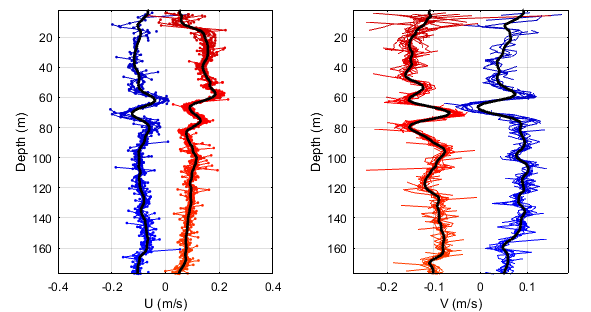
\includegraphics[width=\columnwidth]{./figs/current_profile_snip.png}
  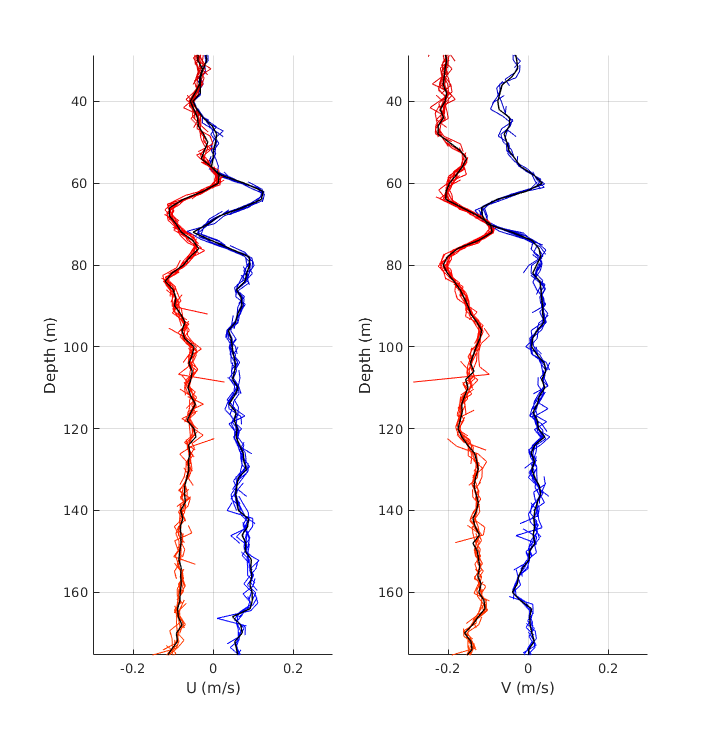
\includegraphics[width=\columnwidth]{./figs/freeprofile_zoom_dv116.png}
  \caption{Overlapping ADCP traces during descent (blue) and ascent (red) for
    dive 99 of sg198, after alignment. The current profile produced by the linear inverse is shown as the thick black line.}
  \label{fig.snippet}
\end{figure}


\begin{figure}
  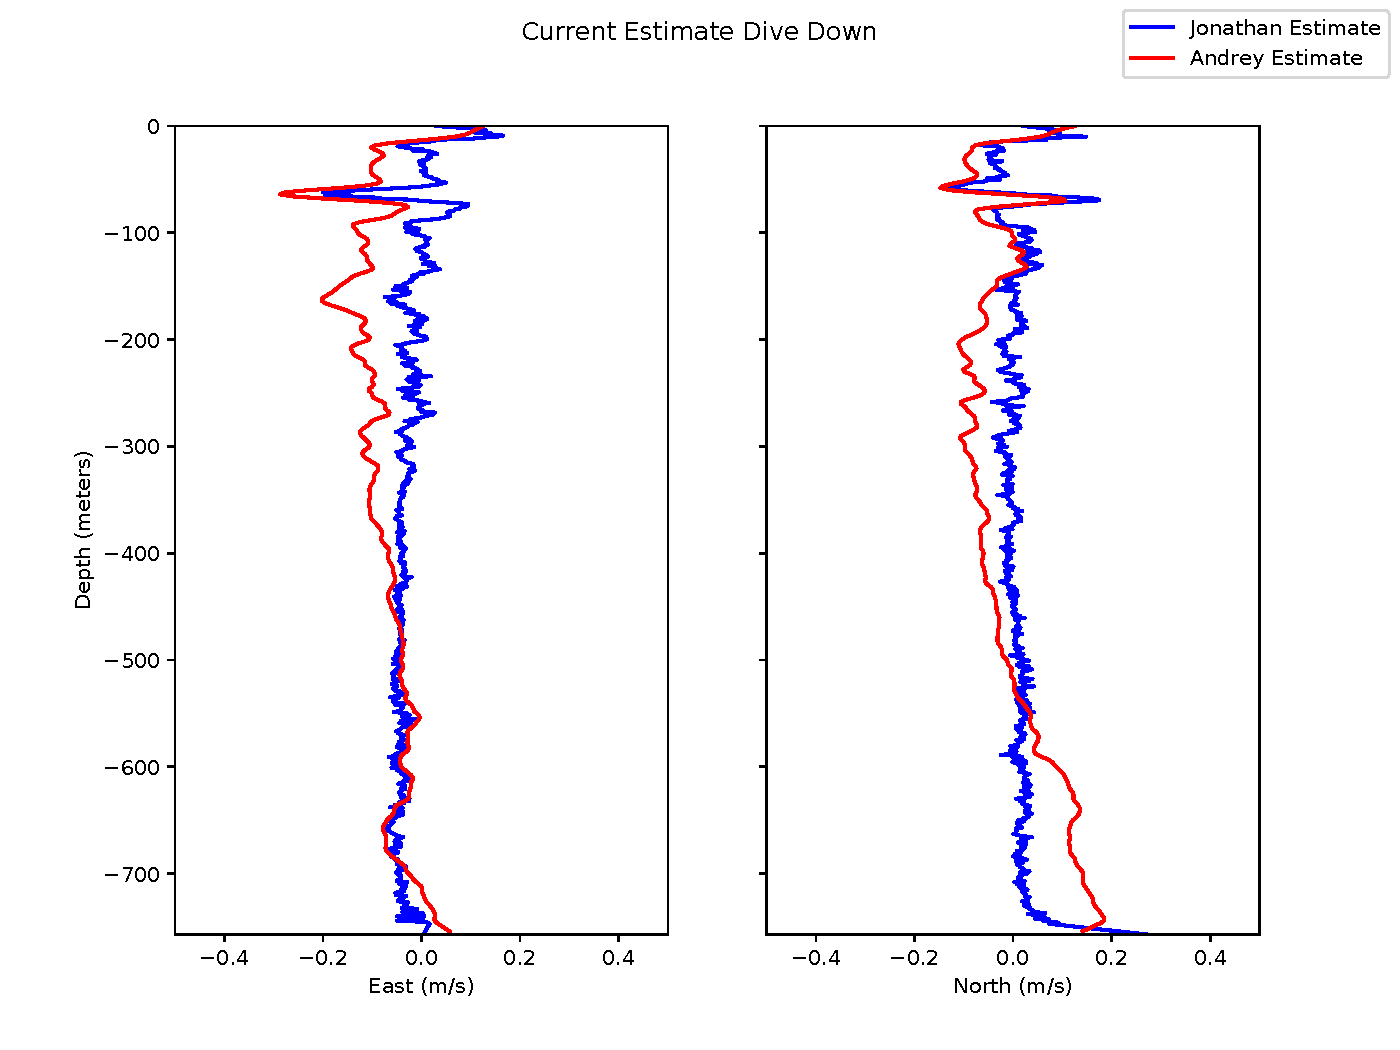
\includegraphics[width=\columnwidth]{./figs/downfull.pdf}
  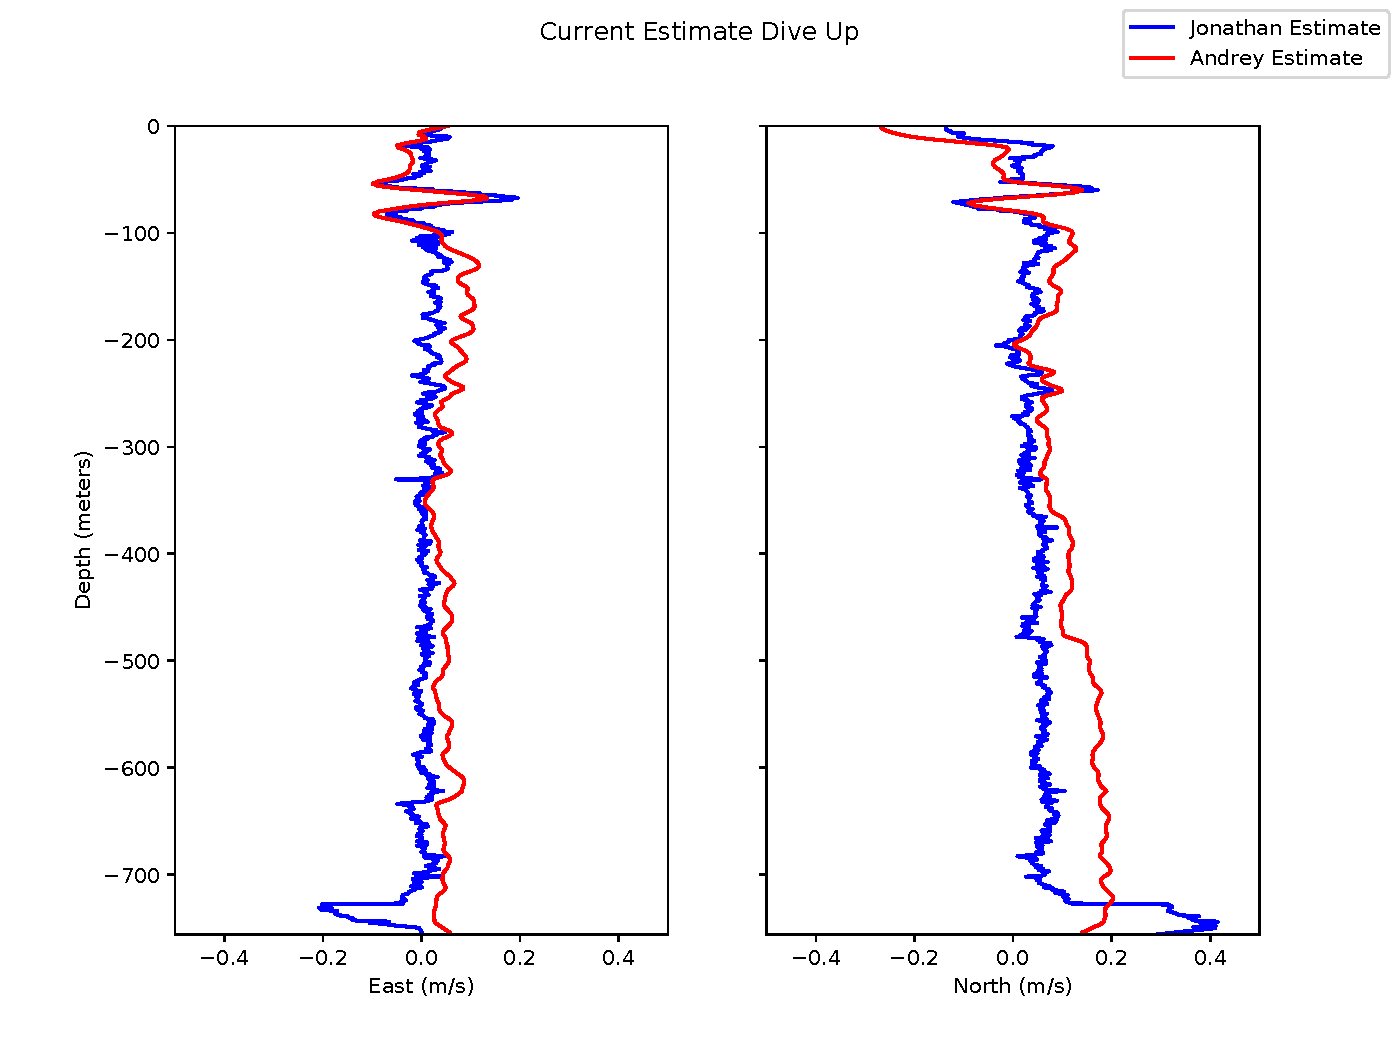
\includegraphics[width=\columnwidth]{./figs/upfull.pdf}
  \caption{The above plot shows a comparison of the results from the linear method compared to the nonlinear method...}
  \label{fig.comparison}
\end{figure}

\begin{figure}%[!ht]
%  \centering
  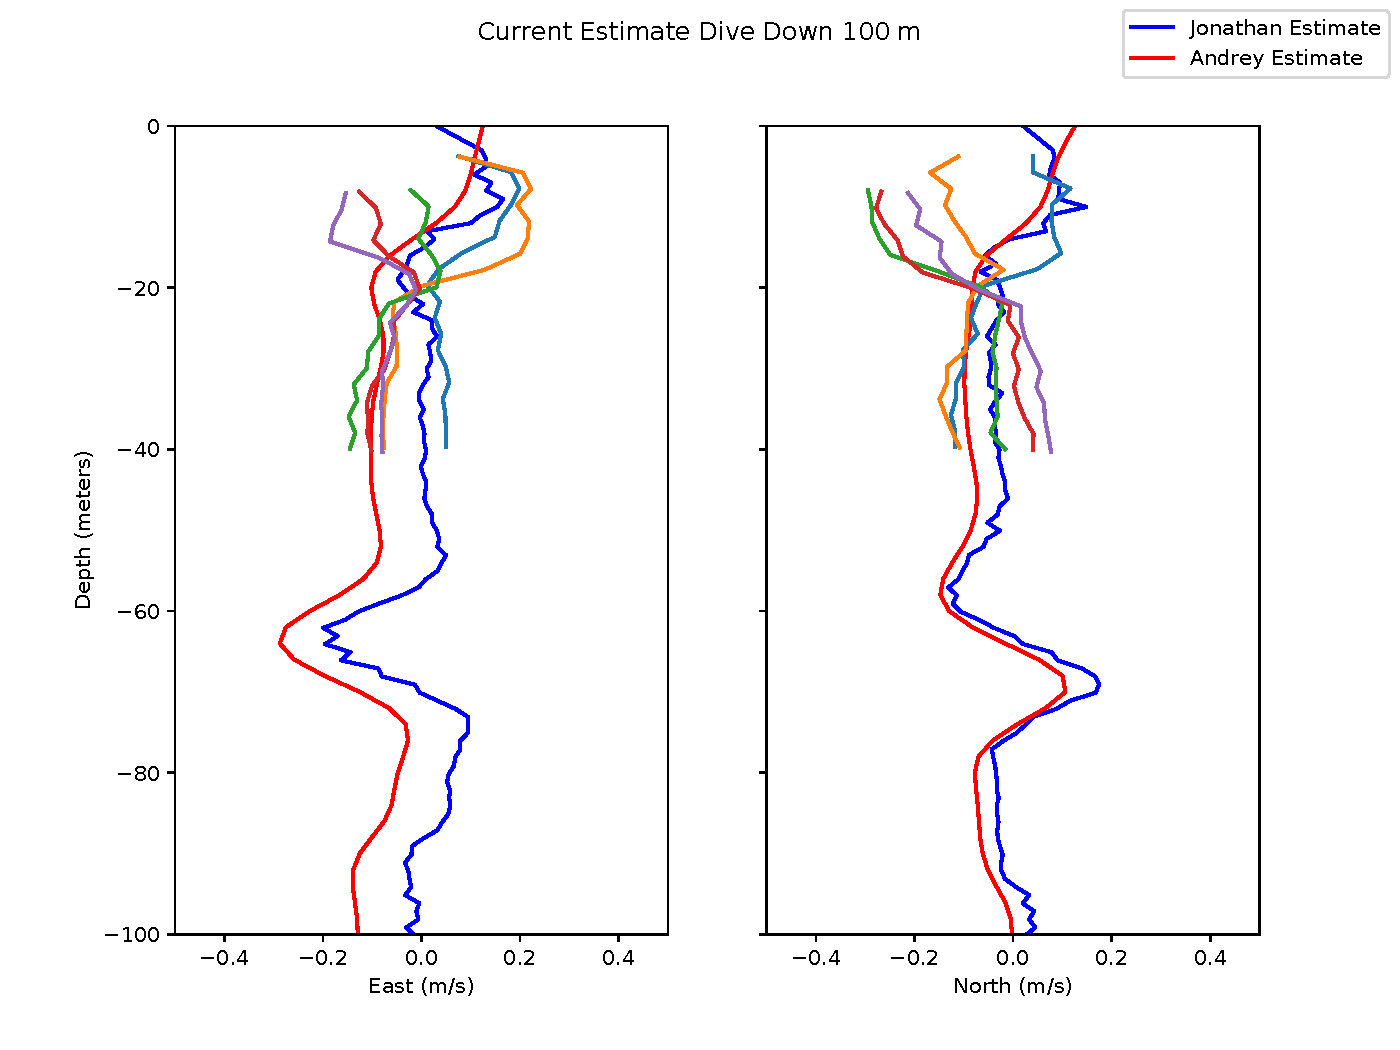
\includegraphics[width=\columnwidth]{./figs/down100.pdf}
  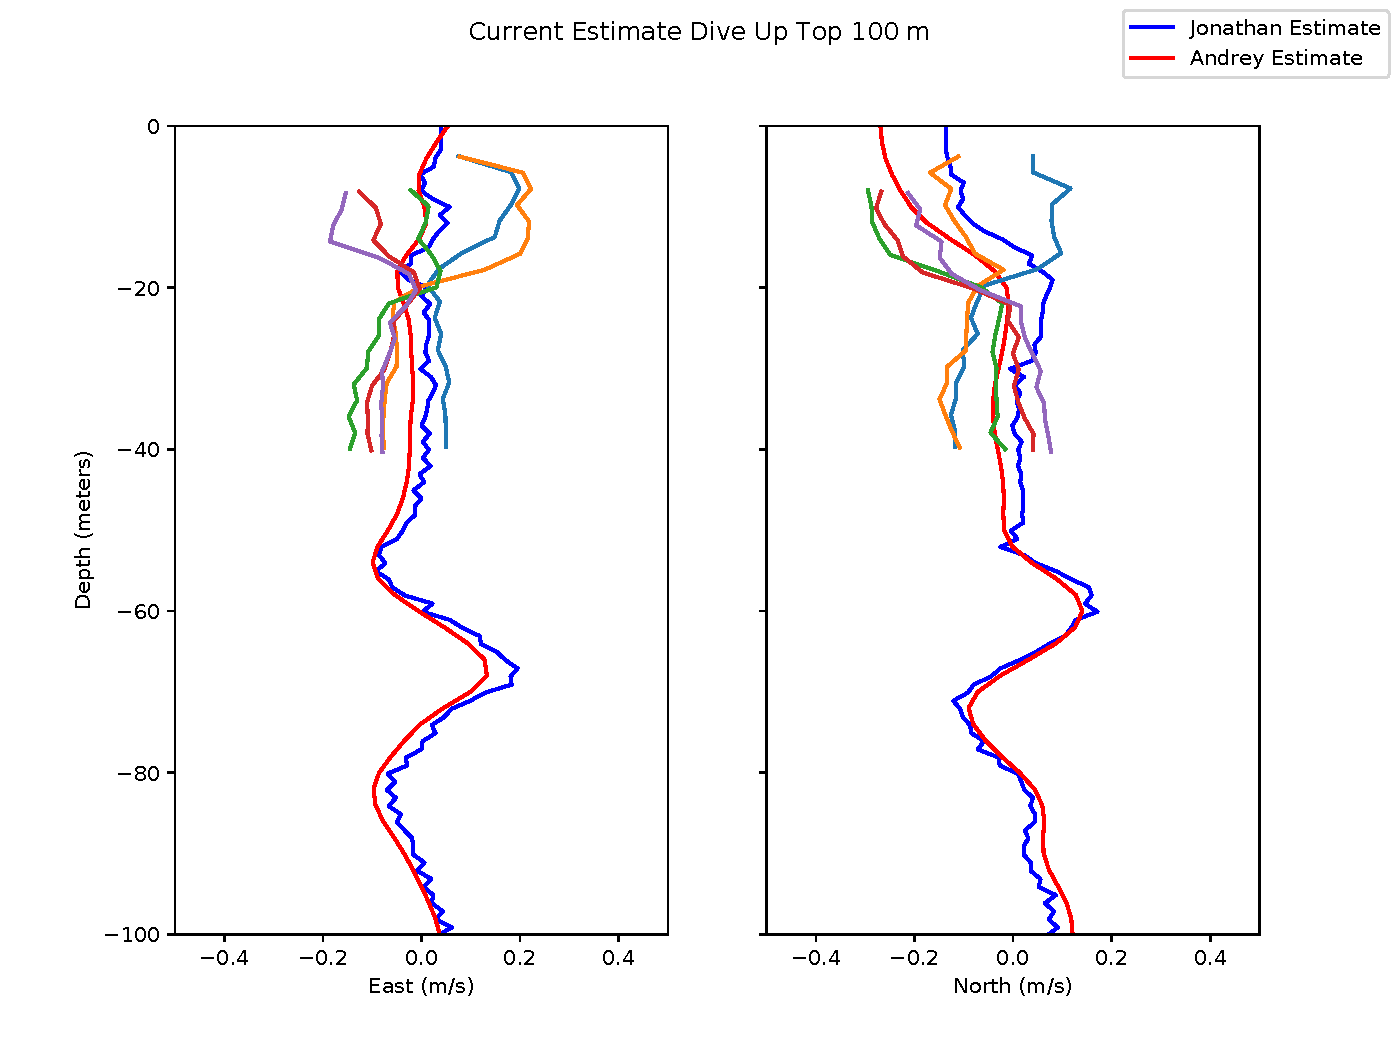
\includegraphics[width=\columnwidth]{./figs/up100.pdf}
  \caption{The above plot shows a comparison between the the linear, nonlinear, and ground truth as obtained from a 600 kHz ADCP on the T3 mooring, which was 13 km away from the glider during this dive.}
  \label{fig.mooring}
\end{figure}






% \begin{figure}[!ht]
%   \centering
%   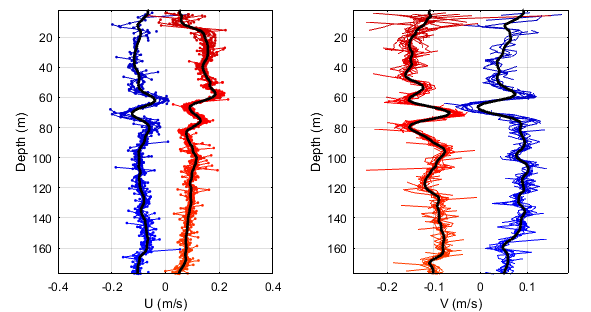
\includegraphics[width=\columnwidth]{./figs/current_profile_snip.png}
%   \vspace{-0.1in}
%   \caption{ Overlapped ADCP profiles during descent (blue) and ascent (red) for dive 116 of sg198. The fitted current profile is shown as the thick black line.}
%   \label{fig.profile_snip}
%   \vspace{-0.1in}
%   %\rule{\textwidth}{0.02in}
% %   \vspace{-0.2in}
% \end{figure}


\section{Conclusions and Future Work \textbf(SASHA)}

- all of the things that we will address

- using a single subsea position fix or multiple subsea range measurements to further constrain the output (I think only the nonlinear model can do this gracefully / easily?)


\section*{Acknowledgements \textbf(SARAH)}
We would like to acknowledge...Ukpik crew...Jason and Craig and Geoff and Ben and Wendy...ONR funding...DRDC funding...Peter and Matt.

